\newpage
\section{Introduction}
\subsection{Motivation}
The company Disruptive Technologies develops and design connected sensing solutions, based on miniature sensors and a software platform for visualization and processing of data. These sensors are battery powered, are extremely small and are connected to the internet via a Sub-GHz adapter. They have a battery lifetime of 15 years with 100 data transactions per day. The size of 19 x 19 x 2 mm and a range of up to 100 m indoors and 1000 m outdoors enables for vast opportunities in both industrial and private applications.   

As of now the company's sensor solutions features touch, proximity and temperature. A useful addition to these sensors would be a image sensor based on Disruptive Technologies platform. This sensor would have to have extremely low power consumption, while take images that are good enough for industrial and/or private applications. It also has to be extremely small, as to keep with Disruptive Technologies design goals and overall market targeting. The target size of the entire minature camera will be 19x19x2mm. 

Among Disruptive Technologies partners are  companies involved in telecommunication, energy, manufacturing and contracting. This includes companies like Powel, Telia and GK Gruppen AS. They have different applications for sensors. Common for them all is that they are interested in energy-efficient, stand-alone sensors that are able to send data wireless. This data can be used for many purposes; automatication, maintanance and surveillance.    

One of the targets of this project thesis is to evaluate if there exists a image-sensor module available on the market today that has the sufficient power consumption, image quality and size to be considered for an ultra-small, ultra low-power camera sensor module. An application study will be done to see what the market wants as of now, and what that would lead to in terms of design requirements. 

\subsubsection{ Internet of Things}
The Internet of Things(IoT) \cite{IoT} provides great opportunities in terms of data gathering and analyzing, automatization, communication and surveillance. As devices and sensors get smaller and more energy efficient, the possibilities for connected, wireless and autonomous systems and sensors in new area of applications arise. The potential is enormous. According to \cite{IoT_devices} the number of IoT devices will be 75.4 billion in 2025, as seen below in \ref{fig:IoT_devices}.
\begin{figure}[H]
\centering
  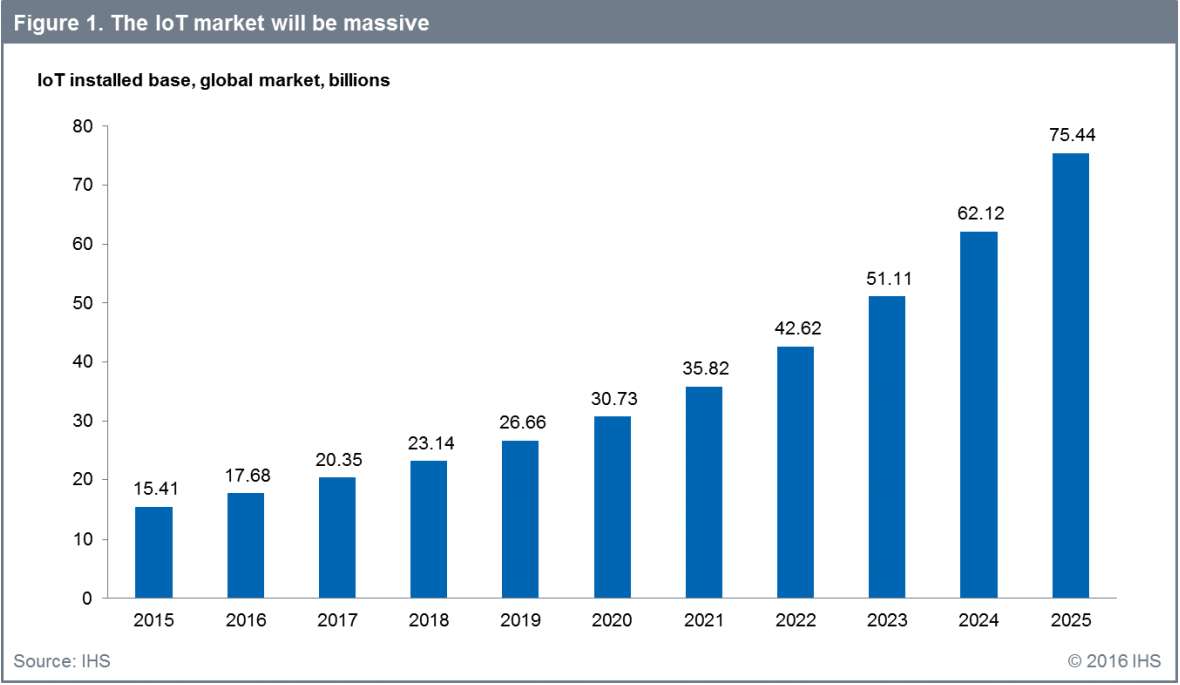
\includegraphics[scale=0.5]{images/iot_number_of_devices.PNG}
  \caption{ Number of installed IoT-devices globally in billions \cite{IoT_devices}. } 
  \label{fig:IoT_devices}
\end{figure}

A miniature camera sensor system, based on Disruptive Technologies platform will be an addition to the already existing growing number of connected devices. The benefit of integrating a miniature camera to Disruptive Technologies platform is the seamless integration of data with the other sensoring solutions from Disruptive Technologies, using the existing software solution.  
As with all other connected devices, security is important. All connected devices can be hacked, either through physical hacking or through software attacks. Many connected devices are developed without enough consideration of security during the development stage. One example is baby monitoring system hacked by Rapid7 \cite{IoT_baby_monitoring}. 
The design of a miniature camera system need to be as secure as possible to prevent unwanted attacks. Disruptive Technologies provide end-to-end cryptation of data through their communication protocol. On-chip attacks will still need to be addressed. This will not be a consideration for the project thesis, but may be continued upon in a master thesis.

\subsection{Current market situation}
Several connected camera monitoring systems exist today. One example is the Netgear Arlo \cite{Net_gear_arlo}. This particular system is designed to have a resolution of 1280x720 pixels, a battery-lifetime at four-six months and are relatively big in size. This camera-system, and others like it, are designed for surveillance. Surveillance require high resolution pictures.
There also exist a lot of connected body-worn cameras. One such example is the Shonin Streamcam\cite{Shonin}. It is battery powered, with a lifetime of about 2,5 hours recording at 720p. 
A comparison of these cameras can be seen in table x below.

%% Insert table here





%% Include some of the alternatives found in market today?

\subsection{Ethical/legal constraints}
All monitoring solutions must abide to strict rules to protect privacy rights. This is especially true for camera monitoring systems with regards to monitoring of peoples activity. According to \cite{datatilsynet_konsesjon}, one must apply for concession if the purpose of monitoring is to register sensitive information like health, sexual information and similar. The strict rules applies to the workplace. According to \cite{datatilsynet_lov} privacy rights makes it hard to monitor employees at work, but concession can be given in order to counter criminal offences and similar. 
\\
For monitoring on private property, the rules are different. It is allowed for a private person to legally monitor his own house and garden. The camera is not allowed to capture parts of public areas or other peoples private property\cite{datatilsynet_lov}. 
\\
For the purpose of surveillance of equipment and machinery, there exist no rules. A miniature camera sensor system would therefore be fitting for such surveillance/monitoring tasks. Due to the nature of monitoring, a concession might be needed due to monitoring people as a bi-product. 
\\
A miniature camera sensor system could therefore be legally used in industrial monitoring of machinery and equipment, as well as in private homes market. 

\subsection{Previous work}
Miniature cameras with extremely low power usage and area have been designed and developed with different purposes. One example is \cite{CMOS Ultra-Low Power}, which is event driven, has a resolution of 64x64 pixels and has a battery lifetime of four months at 5\% duty cycle. It implements on-chip image compression in order to reduce energy consumption. This vision sensor is designed to be used in surveillance and monitoring applications. 
Off-the-shelf HW solutions for surveillance and monitoring applications has been implemented in \cite{Off_the_shelf_HW}. The solution proposed in this paper is not to be considered ultra small, as it uses a Raspberry Pi(Rpi) and a Libellium Waspmote platform. The power consumption is quite high(in the range of Watts) compared to the desired specifications of a miniature camera. 
The NanEye2D image module \cite{NanEye_datasheet} has been used in various setups for different applications, including as a standalone image module\cite{Eyes_of_things_NanEye} and for 3D-imaging\cite{NanEye_3D}. It is designed for medical endoscopy applications. The low power consumption and extremely low size makes it usable for miniature-camera applications.  

\section{Paper Overview}
The following chapers in this project report delve into the integration of a miniature camera on a Disruptive Technology sensor. Different image sensor modules will be considered, with respect to applications and the following specifications set by different applications.  

Chapter 2 is the Theory

Chapter 3 is the Applications

...


